%%%%%%%%%%%%%%%%%%%%%  kbb talk %%%%%%%%%%%%%%%%%%%%%%%%%%%%%%%
%%%%%%%%%%%%%%%%%%%%%%%%%%%%%%%%%%%%%%%%%%%%%%%%%%%%%%%%%%%%%%%

\documentclass[12pt,fleqn]{seminar}
\input{seminar.bug}
\pagestyle{empty}
\pdfhorigin=1truein
\pdfvorigin=1truein


% packages
\usepackage{ifpdf}
\usepackage{bm}
\usepackage{latexsym}
\usepackage{color}
\usepackage{pstricks}
\usepackage{ulem} %uwave
\usepackage{amsmath}

\usepackage{amssymb}
%\usepackage{float}
\usepackage{bm}
%\usepackage{wasysym}
%\usepackage[landscape]{geometry}
\usepackage{graphicx}
\usepackage{epstopdf}
\graphicspath{{./Figs/}{./}{../}}

\begin{document}


% basic	commands I
\newcommand{\mass}{\mathsf{M}} 
\newcommand{\half}{\mbox{\small $\frac{1}{2}$}}
\newcommand{\sinc}{\mbox{sinc}}
\newcommand{\const}{\mbox{const}}
\newcommand{\trc}{\mbox{trace}}
\newcommand{\intt}{\int\!\!\!\!\int }
\newcommand{\ointt}{\int\!\!\!\!\int\!\!\!\!\!\circ\ }
\newcommand{\eexp}{\mbox{e}^}
\newcommand{\bra}{\left\langle}
\newcommand{\ket}{\right\rangle}
\newcommand{\EPS} {\mbox{\LARGE $\epsilon$}}
\newcommand{\ttimes} {\mbox{\tiny \ $^{\times}$ \ }}
\newcommand{\ar}{\mathsf r}
\newcommand{\im}{\mbox{Im}}
\newcommand{\re}{\mbox{Re}}
\newcommand{\bmsf}[1]{\bm{\mathsf{#1}}} 
\newcommand{\pd}[2]{\frac{\partial #1}{\partial #2}}
\newcommand{\bitem}{$\newline \ \ \bullet \ \ $} 
\newcommand{\ola}{\protect\overleftarrow}
\newcommand{\ora}{\protect\overrightarrow}

% basic	commands II
\newcommand{\hide}[1]{}
\newcommand{\tbox}[1]{\mbox{\tiny #1}}
\newcommand{\Cn}[1]{\begin{center}{#1}\end{center}}
\newcommand{\be}{\begin{eqnarray*}}
\newcommand{\ee}{\end{eqnarray*}}
\newcommand{\beq}{\begin{eqnarray*}}
\newcommand{\eeq}{\end{eqnarray*}}

\newcommand{\mpg}[2][0.45\hsize]{\begin{minipage}[b]{#1}{#2}\end{minipage}}
%
\newcommand{\bmp}[1]{\begin{minipage}[t]{#1}\noindent }
\newcommand{\smp}[1]{\end{minipage}\begin{minipage}[t]{#1}\noindent }
\newcommand{\emp}{\end{minipage}}

\newcommand{\amatrix}[1]{\begin{matrix} #1 \end{matrix}} 


% extra commands for colors
\definecolor{blk}{rgb}{0.,0.,0.}
\definecolor{red}{rgb}{1.,0.,0.}
\definecolor{green}{rgb}{0.,0.5,0.}
\definecolor{blue}{rgb}{0.,0.,1.}
\definecolor{bluek}{rgb}{0.,0.,0.5}
\definecolor{orange}{rgb}{1.,0.56.,0}
\newcommand{\cblk}[1]{\textcolor{blk}{#1}}
\newcommand{\cred}[1]{\textcolor{red}{#1}}
\newcommand{\cgreen}[1]{\textcolor{green}{#1}}
\newcommand{\cblue}[1]{\textcolor{blue}{#1}}
\newcommand{\cbluek}[1]{\textcolor{bluek}{#1}}
\newcommand{\corange}[1]{\textcolor{orange}{#1}}


% extra commands for slides

%\newcommand{\Up}[1][0.5]{\vspace{-#1cm}}
%\newcommand{\Dn}[1][0.5]{\vspace{#1cm}}
%\newcommand{\Tl}[1]{\begin{center}{\bf \small \cblue{#1}}\end{center}}

\newcommand{\Up}[1][5]{\vspace{-#1mm}}
\newcommand{\Dn}[1][5]{\vspace{#1mm}}
\newcommand{\Tl}[1]{\begin{center}{\bf \small \cblue{#1}}\end{center}}

\renewcommand{\slideparindent}{0mm}
\setlength{\mathindent}{0cm} 

% \newcommand{\newsld}{\end{slide}\begin{slide}}


\newcommand{\bslA}[1]{
%portrait
\pdfpagewidth=210truemm
\pdfpageheight=297truemm
\pdfhorigin=1truein
\pdfvorigin=1truein
%portrait
\renewcommand{\slidetopmargin}{0mm}
\renewcommand{\slideleftmargin}{-54mm}
\setlength{\slidewidth}{190mm}
\setlength{\slideheight}{277mm}
\begin{slide}
}



\newcommand{\bslB}[1]{
%landscape
\pdfpagewidth=297truemm
\pdfpageheight=210truemm
\pdfhorigin=1truein
\pdfvorigin=1truein
%portrait 
\renewcommand{\slidetopmargin}{0mm}
\renewcommand{\slideleftmargin}{33mm}
\setlength{\slideheight}{190mm}
\setlength{\slidewidth}{150mm} %130
%portrait fonts
\begin{slide}
\ptsize{8}
}



\newcommand{\bslC}[1]{
%landscape
\pdfpagewidth=297truemm
\pdfpageheight=210truemm
\pdfhorigin=1truein
\pdfvorigin=1truein
%landscape
\renewcommand{\slidetopmargin}{0mm}
\renewcommand{\slideleftmargin}{33mm}
\setlength{\slideheight}{190mm}
\setlength{\slidewidth}{277mm}
%portrait fonts
\begin{slide}
\ptsize{8}
}



\newcommand{\bslD}[1]{
%landscape
\pdfpagewidth=297truemm
\pdfpageheight=210truemm
\pdfhorigin=1truein
\pdfvorigin=1truein
%landscape
\renewcommand{\slidetopmargin}{0mm}
\renewcommand{\slideleftmargin}{33mm}
\setlength{\slideheight}{190mm}
\setlength{\slidewidth}{277mm}
%landscape fonts
\begin{slide}
}



\newcommand{\esl}{\end{slide}}


\newcommand{\vbar}{
\begin{picture}(1,1)
\thicklines
\put(0,61){ \ \ \line(0,-1){280} \ \ } 
\end{picture} 
}


%%%%%%%%%%%%%%%%%%%%%%%%%%%%%%%%%%%%%%%%%%%%%%%%%%%%%%%%%%%%%%%%%%%
%%%%%%%%%%%%%%%%%%%%%%%%%%%%%%%%%%%%%%%%%%%%%%%%%%%%%%%%%%%%%%%%%%%


%%%%%%%%%%%%%%%%%%%%%%%%%%%%%%%%%%%%%%%%%%%%%%%%%%%%%%%%%%%%%%%%%%%
%%%%%%%%%%%%%%%%%%%%%%%%%%%%%%%%%%%%%%%%%%%%%%%%%%%%%%%%%%%%%%%%%%%

%%%%%%%%%%%%%%%%%%%%%%%%%%%%%%%%
\bslD

\Tl{\Large{Percolation, sliding, localization and relaxation in glassy circuits }}


\Cn{\bf Daniel Hurowitz, Doron Cohen,\\ \corange{Ben-Gurion University}}
%
%
%\bmp{0.5\hsize}
%
%
%
%%\Cn{ \includegraphics[ height=4cm]{}}
%
%\smp{0.5\hsize}
%
%\vspace{0.2cm}
%
%
%
%%{\includegraphics[height=3cm]{ResistorsNetworkBath_a}}
%
%\emp
%
%\bmp{\hsize}



\bmp{0.5\hsize}

\Cn{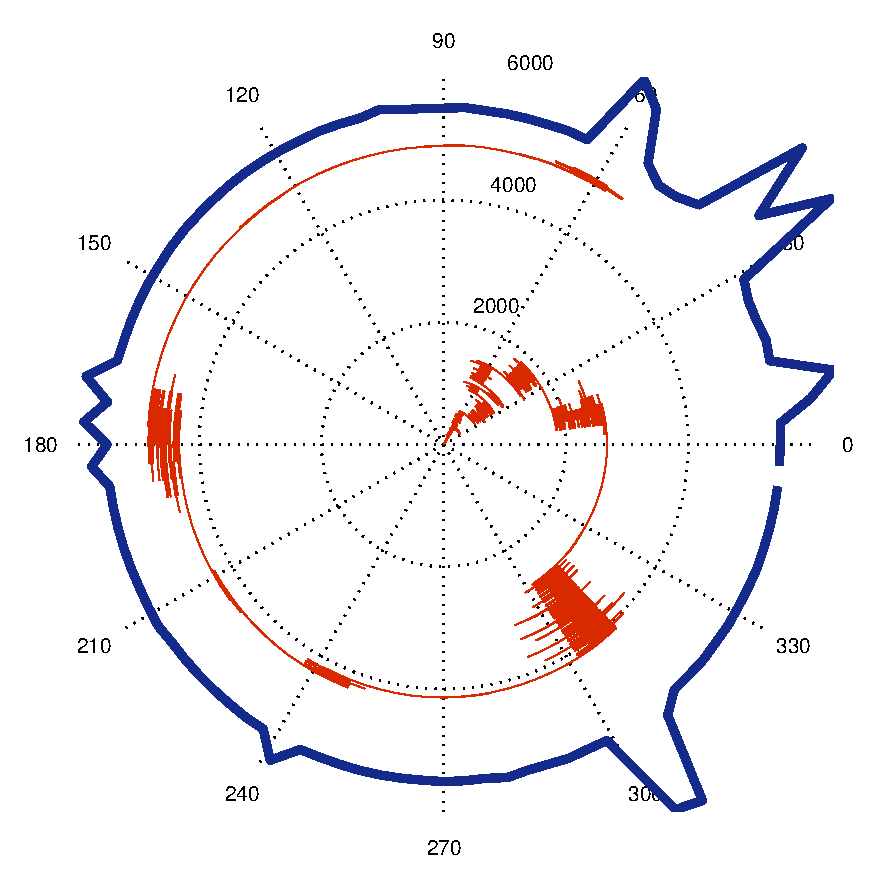
\includegraphics[height=5cm]{/Figs/polar_1_a.eps}}

\smp{0.5\hsize}

\Cn{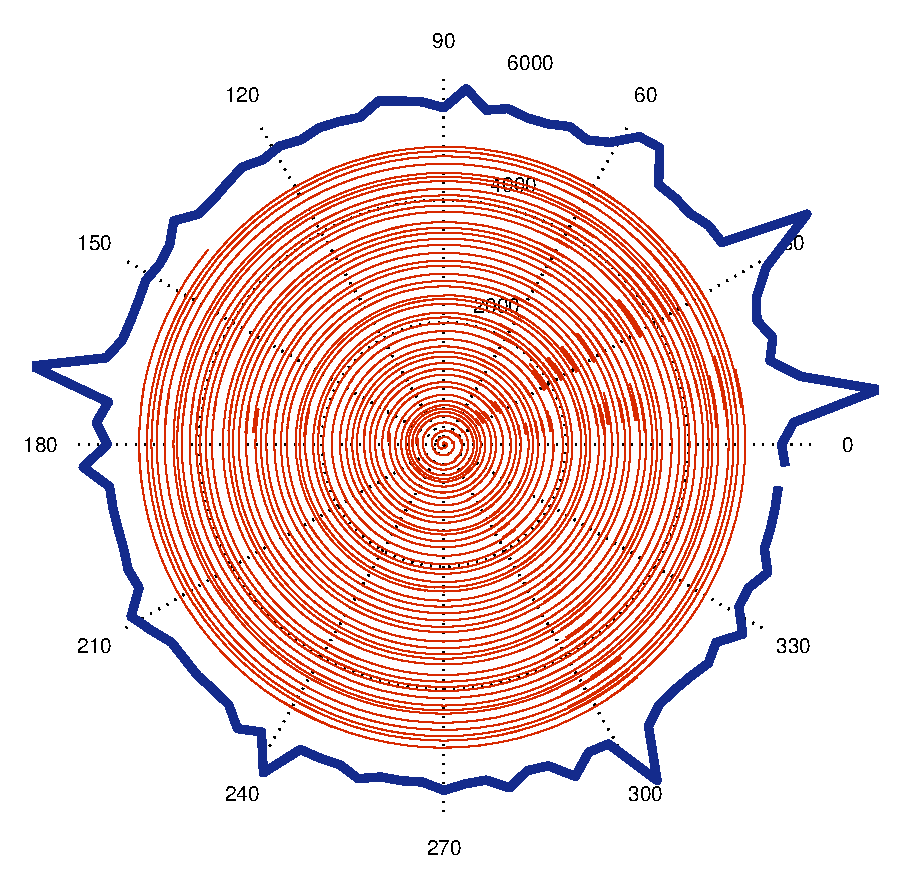
\includegraphics[height=5cm]{/Figs/polar_2_a.eps}}

\emp



%\emp

\esl


%%%%%%%%%%%%%%%%%%%%%%%%%%%%%%%%
\bslC

\Tl{\large Brownian motion}

\Dn[2]

\cgreen{The Einstein-Smoluchowski Relation (ESR):}

\Up

\beq
\hspace{5cm} D = \mu k_B T, \ \ \ \ \ \ \ \ \ \ k_B=1
\eeq

Relation between mobility ($\mu$) and diffusion ($D$) reflecting microscopics ($k_B$) in universal way.

This is a special case of a \cred{fluctuation-dissipation relation} between first and second moments.



\beq
\text{\cgreen{Drift:}} \ \  && \langle x \rangle \ = \ vt, \ \ \ \ \ \ \  v \ = \ \mu F  \\
\text{\cgreen{Diffusion:}} \ \  && \text{Var}(x) \ = \ 2Dt \\
\text{\cgreen{ESR:}} \ \ && \frac{v}{D} \ \ = \ \  \frac{F}{T} \ \ \equiv \ \ s \ \ = \ \ \mbox{\cgreen{affinity (linear response)}}
%\ \ \ \ \ \cgreen{\leadsto} \ \ \ \ \  \frac{\mu}{D} \ = \ \frac{1}{T}
\eeq

\Dn

$s \ \equiv \ $ \cgreen{entropy-production-per-distance}  

\Dn

\center{\cred{\bf FDT is valid close to equilibrium.}}

\center{\cred{\bf To what extent does the ESR hold? }}

\center{\cred{\bf Can it be derived from the NFT? }}

\center{\cred{\bf Non-equilibrium version?}}

\esl


%%%%%%%%%%%%%%%%%%%%%%%%%%%%%%%%%%%%%%%%%%
\bslC

\Tl{Percolation}

\esl

%%%%%%%%%%%%%%%%%%%%%%%%%%%%%%%%%%%%%%%%%%
\bslC

\Tl{Sinai spreading}

\esl


%%%%%%%%%%%%%%%%%%%%%%%%%%%%%%%%%%%%%%%%%%
\bslC

\Tl{Localization}

\esl

\end{document}


